\begin{figure}[h!]
    \centering
    \caption{Estimated shares pocketed by landlords under counterfactual MW policies}
    \label{fig:cf_hist_shares}

    \begin{subfigure}{0.65\textwidth}
        \caption{Increase in federal MW to \$9, urban ZIP codes}
        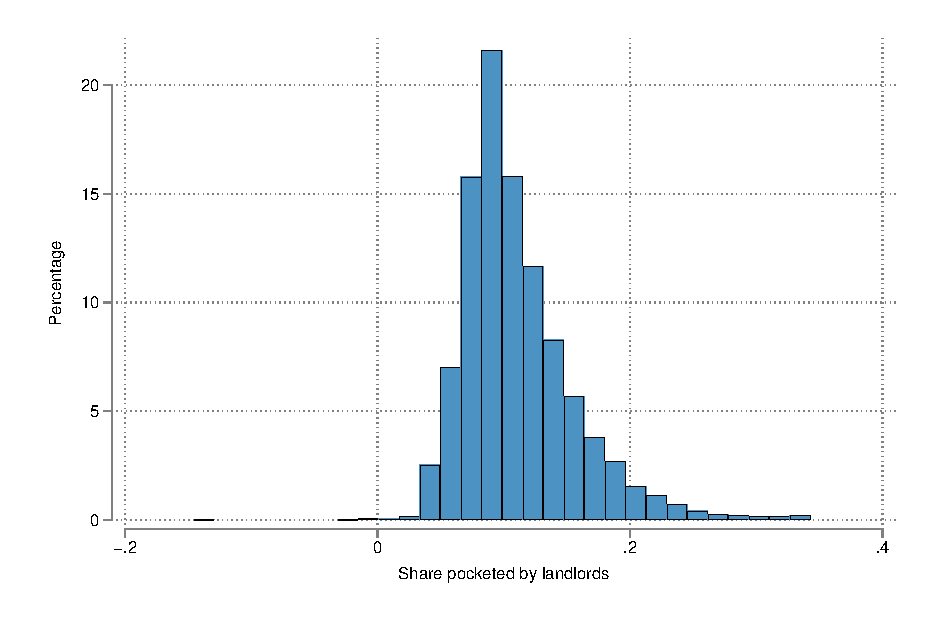
\includegraphics[width = 1\textwidth]{counterfactuals/output/hist_rho_with_imputed_fed_9usd}
    \end{subfigure}

    \begin{subfigure}{0.65\textwidth}
        \caption{Increase in Chicago MW to \$14, Chicago-Naperville-Elgin CBSA}
        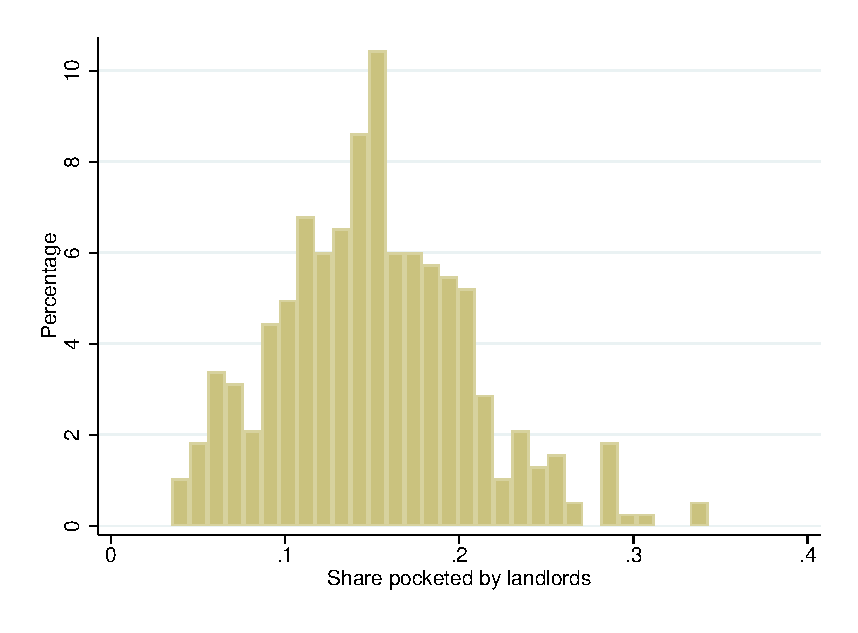
\includegraphics[width = 1\textwidth]{counterfactuals/output/hist_rho_with_imputed_chi14}
    \end{subfigure}

    \begin{minipage}{.95\textwidth} \footnotesize
        \vspace{3mm}
        Notes:
        Data are from the MW panel described in section \ref{sec:data_mw_panel} 
        and from LODES.
        The figures show the distribution of the estimated ZIP-code specific
        shares of the additional income pocketed by landlords (``share pocketed'')
        under different counterfactual policies.
        Panel (a) is based on a counterfactual increase to \$9 in the 
        federal MW in January 2020, holding constant other MW policies in their 
        December 2019 levels.
        Panel (b) is based on a counterfactual increase from \$13 to \$14 in the 
        Chicago City MW, also holding constant other MW policies.
        The unit of observation is the ZIP code.
        Panel (a) includes ZIP codes located in urban CBSAs where the estimated 
        increase in income was higher than 0.1\%.
        Panel (b) includes ZIP codes in the Chicago-Naperville-Elgin CBSA.
        The share pocketed is defined as the ratio between the percent increase 
        in rents and the percent increase in total wages multiplied by the share 
        of housing expenditure in the ZIP code.
        To estimate it we follow the procedure described in Section 
        \ref{sec:counterfactual}, assuming the following parameter values: 
        $\beta = \betaCf$, $\gamma = \gammaCf$, and $\varepsilon = \epsilonCf$.
    \end{minipage}
\end{figure}
